\documentclass[12pt]{article}
\usepackage[margin=1in]{geometry}                % See geometry.pdf to learn the layout options. There are lots.
\geometry{letterpaper}                   % ... or a4paper or a5paper or ... 
%\geometry{landscape}                % Activate for for rotated page geometry
\usepackage[parfill]{parskip}    % Activate to begin paragraphs with an empty line rather than an indent

%%%%%%%%%%%%%%%%%%%%
\newcommand{\hide}[1]{}



\usepackage{natbib}
\usepackage{xcolor}
\usepackage{url}
\usepackage{hyperref}
\usepackage{mathtools}
\usepackage[utf8]{inputenc}
\usepackage{float}
\usepackage{listings}
\usepackage{xcolor}
\usepackage{seqsplit}
\usepackage{verbatim}


\hide{
\usepackage{amscd}
\usepackage{amsfonts}
\usepackage{amsmath}
\usepackage{amssymb}
\usepackage{amsthm}
\usepackage{cases}		 
\usepackage{cutwin}
\usepackage{enumerate}
\usepackage{enumitem}
\usepackage{epstopdf}
\usepackage{graphicx}
\usepackage{ifthen}
\usepackage{lipsum}
\usepackage{mathrsfs}	
\usepackage{multimedia}
\usepackage{wrapfig}
}
\bibliographystyle{humanbio}


\usepackage[utf8]{inputenc}

\newcommand{\itemlist}[1]{\begin{itemize}#1\end{itemize}}
\newcommand{\enumlist}[1]{\begin{enumerate}#1\end{enumerate}}
\newcommand{\desclist}[1]{\begin{description}#1\end{description}}
\newcommand\tab[1][0.5cm]{\hspace*{#1}}

\newcommand{\Answer}[1]{\begin{quote}{\color{blue}#1}\end{quote}}
\newcommand{\AND}{\wedge}
\newcommand{\OR}{\vee}
\newcommand{\ra}{\rightarrow}
\newcommand{\lra}{\leftrightarrow}

\title {{\bf ECE 471 Lab 5} \\
\large{Packet Sniffing and Spoofing Lab / ARP Cache Poisoning Attack Lab
}}

\author{Mitchell Dzurick}
\date{4/15/2020}
\begin{document}

\maketitle
\textbf{Github with all documentation - \url{https://www.github.com/mitchdz/ECE471}}
\tableofcontents 
\clearpage



\section{Packet Sniffing and Spoofing Lab}

\subsection{Task 1.1: Sniffing Packets}
\subsubsection{Task 1.1A}
The program is created below:
\begin{verbatim}
#!/usr/bin/python
from scapy.all import *

def print_pkt(pkt):
    pkt.show()

pkt = sniff(filter=’icmp’,prn=print_pkt)

\end{verbatim}

This code is placed into a file named sniffing.py and made executable with the following command

\begin{verbatim}
$ sudo chown +x sniffing.py
\end{verbatim}
The code can then be ran with the following command
\begin{verbatim}
$ ./sniffing.py
\end{verbatim}

The output is as follows:
\begin{figure}[H]
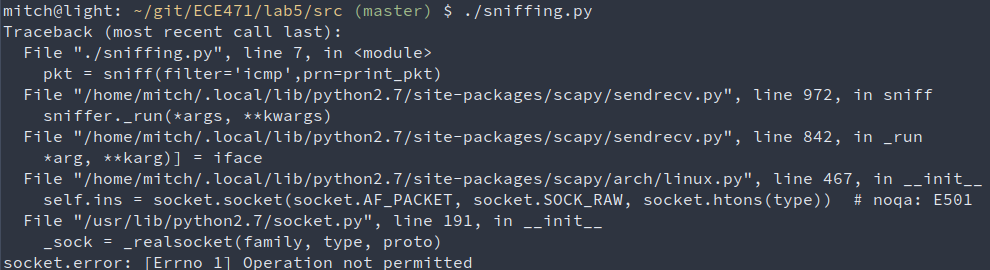
\includegraphics[scale=0.45]{images/p1t1_1.png}
\caption{Running the sniffing program without root}
\label{fig:p1t1_1}
\end{figure}





\subsubsection{Task 1.1b}

\subsection{Task 1.2: Spoofing ICMP Packets}
\subsection{Task 1.4: Sniffing and-then Spoofing (Extra Credit)}

\section{ARPCache Poisoning Attack Lab}
\subsection{Task 2.1: ARP Cache Poisoning}





\end{document}

